\chapter{Testing}
\label{ch:testing}
\section{Introduction}
This section documents the testing phase of the project. In order to establish whether the system is successful or not, we must test the system against the initial requirements outlined in Section~\ref{sec:requirements}. We must also check whether the users accept the final solution. For this chapter there are three stages to testing:

\begin{itemize}
	\item Requirements Testing - Testing each requirement from the requirements specification and giving evidence whether the requirement was fulfilled.
	\item System Testing - Testing the system as a whole, evaluating the accuracy and efficacy of the application. This stage has involvement from the test users.
	\item User Acceptance Testing - Ensuring that each user accepts the solution. Feedback is provided by each user, as well as suggested future work.
\end{itemize}

The next section gives evidence for the requirements testing.

\newpage

\begin{landscape}
	\section{Requirements Testing}
	\subsection{Functional Requirements}
	\begin{tabularx}{\hsize}{lXXXr}
		\toprule
		ID & Name & Expected Output & Evidence & Success? \\
		\midrule
		F1 & User Interaction 
		& A page should display to allow the user to interact with the bot
		& 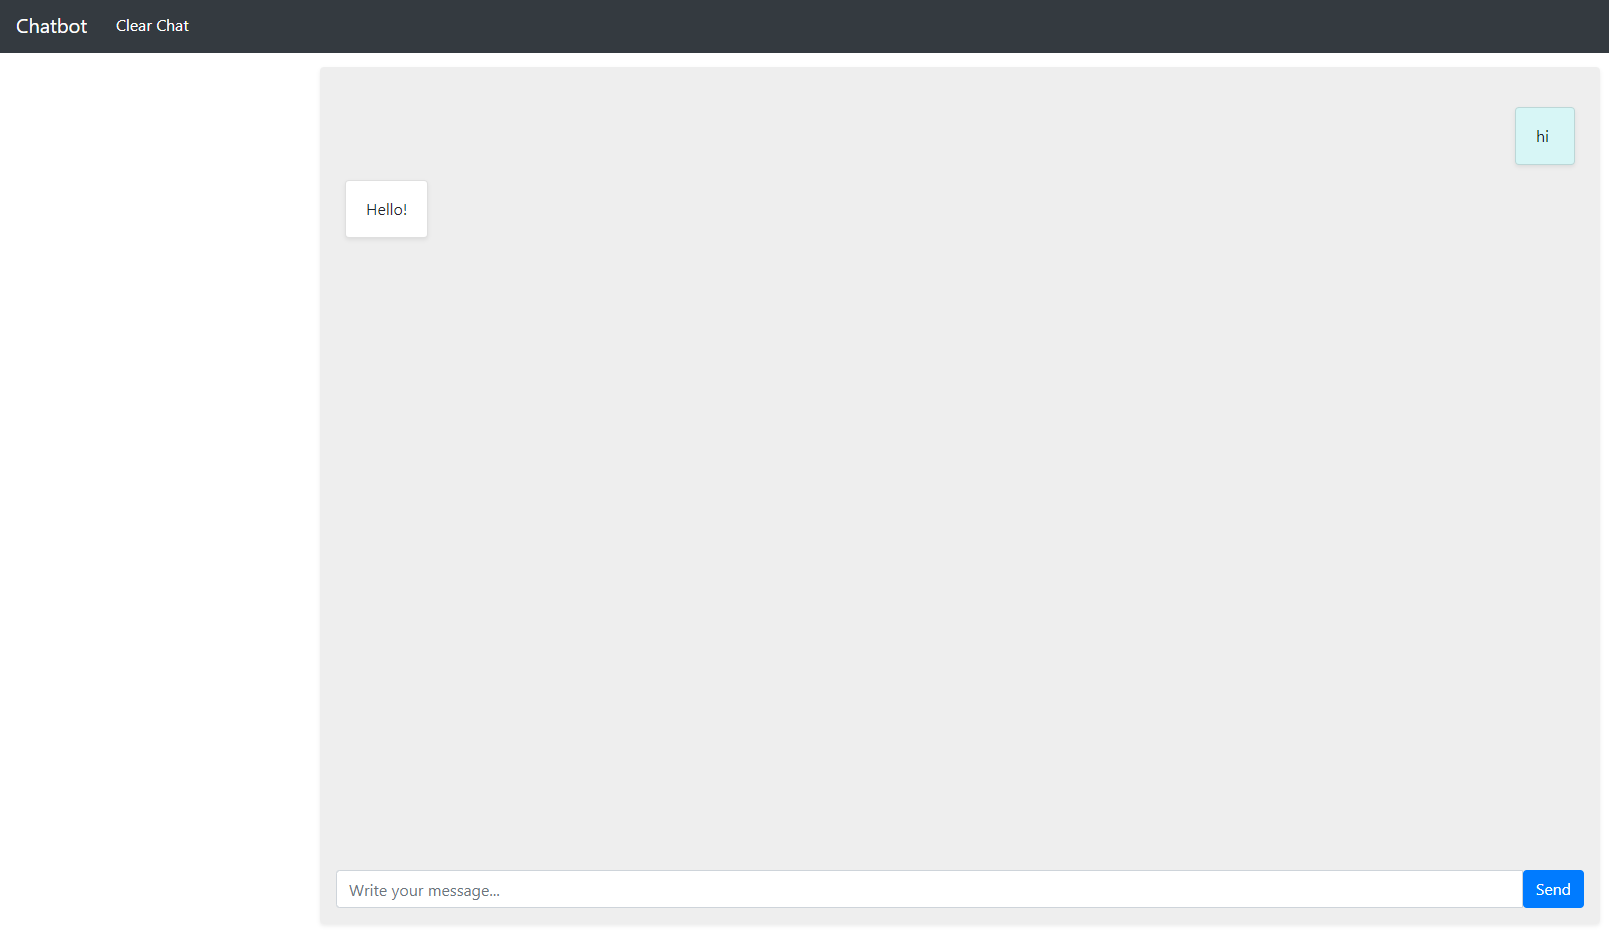
\includegraphics[width=8cm, valign=m]{tests/f1} & Yes \\
		\midrule
		F2 & Browser Access
		& The user should be able to access the system via a browser
		& 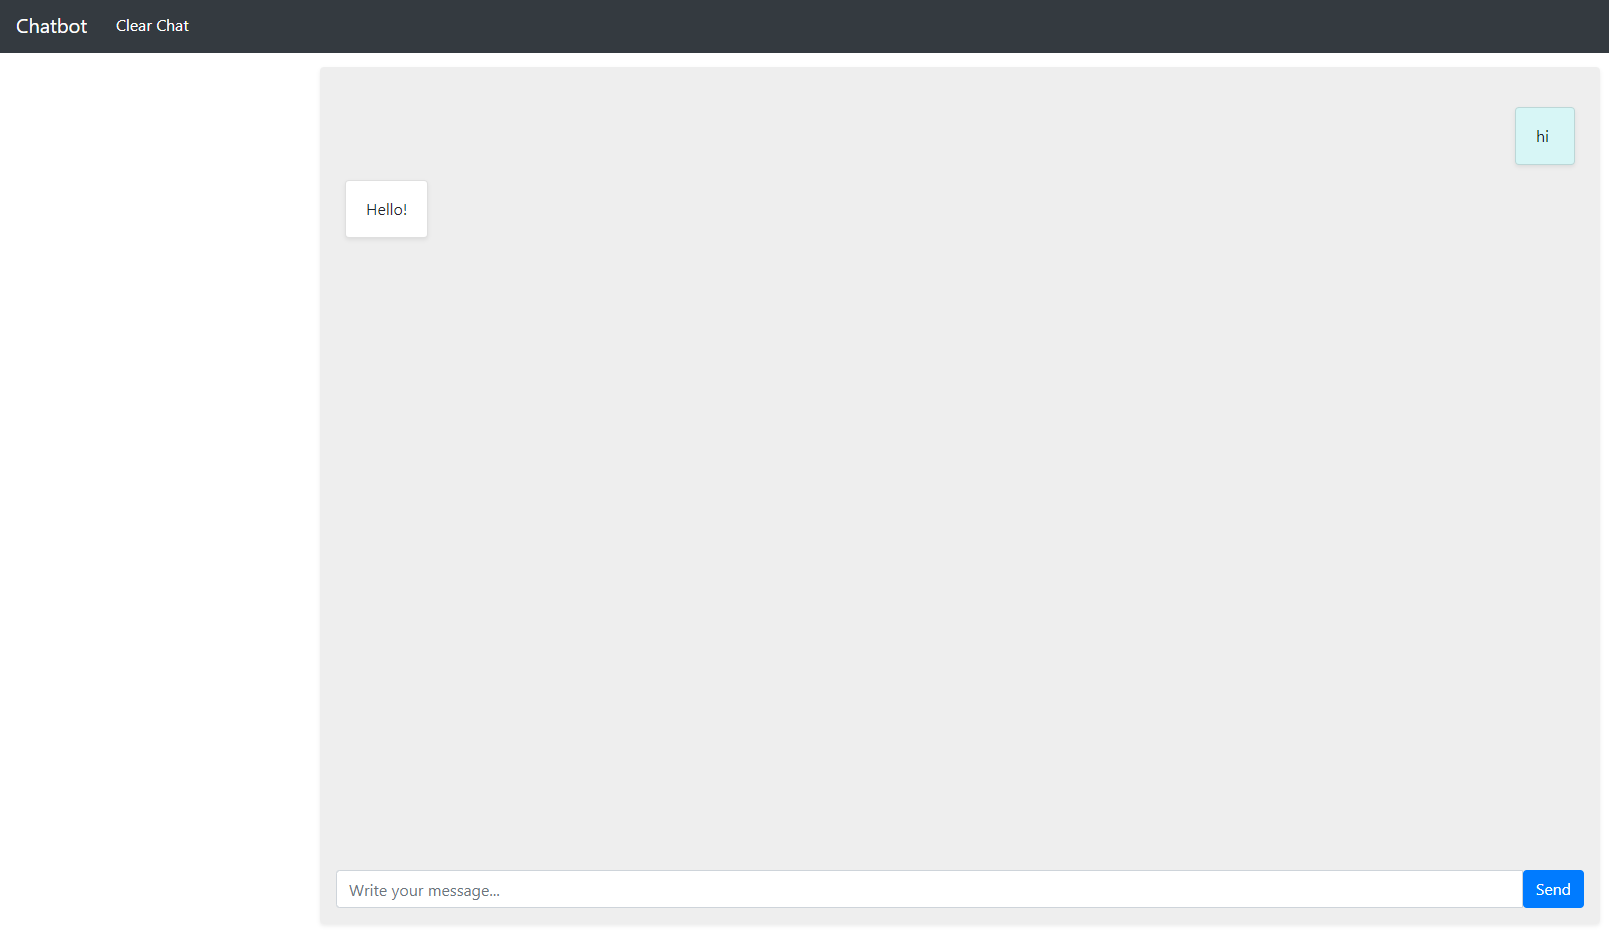
\includegraphics[width=8cm, valign=m]{tests/f1} & Yes \\
		\midrule
		F3 & User Input
		& The user should be enter queries to the bot using a textbox input
		& 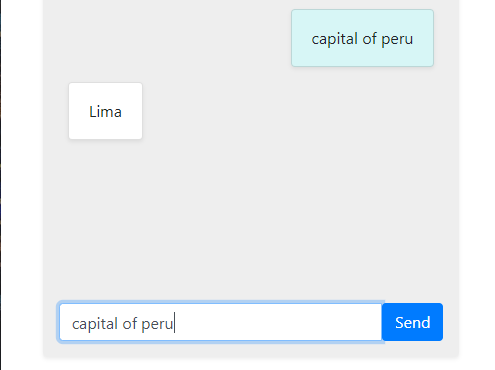
\includegraphics[width=8cm, valign=m]{tests/f3} & Yes \\
		\midrule
		F4 & Responses on Page
		& The should see the chatbot response on the web page
		& 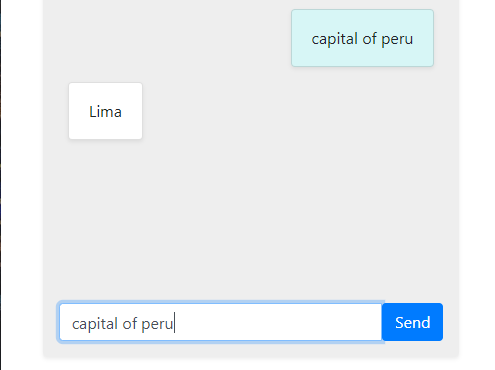
\includegraphics[width=8cm, valign=m]{tests/f3} & Yes \\
		\midrule
		F5 & Conversation History
		& The should see the whole conversation with the bot on the page
		& 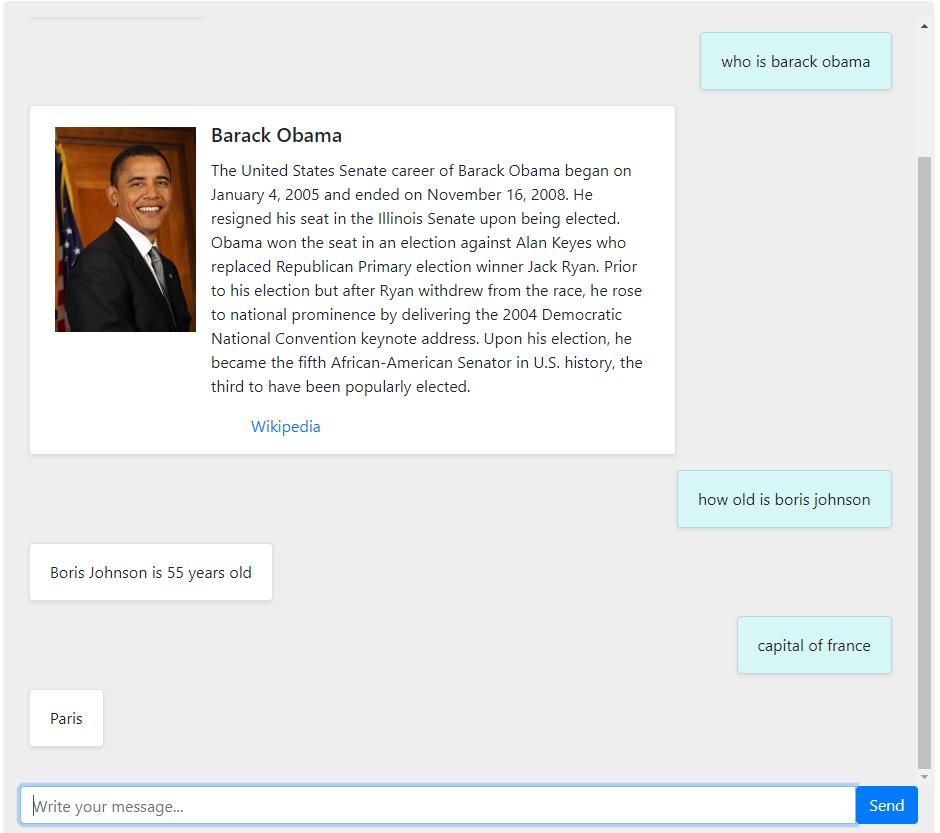
\includegraphics[width=8cm, valign=m]{tests/f5} & Yes \\
		\midrule
		F6 & Person Description Query
		& The user should be able to ask a query about who a person is\newline - 'WHO IS *' and receive a description of that person
		& 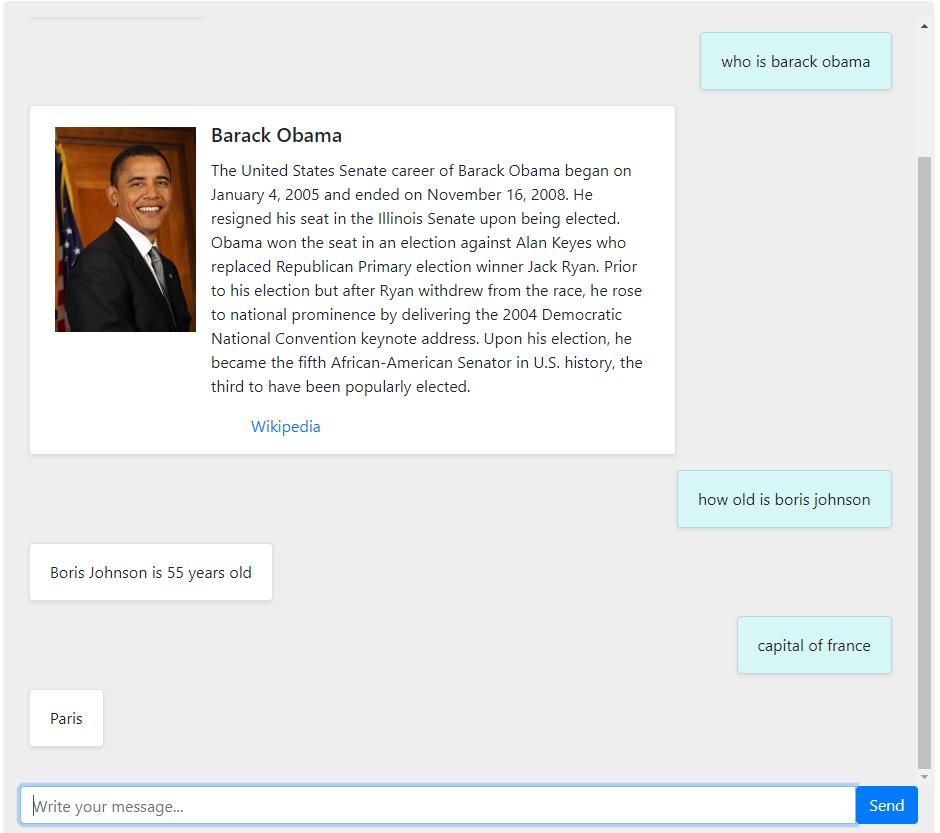
\includegraphics[width=8cm, valign=m]{tests/f5} & Yes \\
		\midrule
		F7 & Person Birthdate Query
		& The user should be able to ask a query about when a person was born\newline - 'WHEN WAS * BORN' and see their birth date
		& 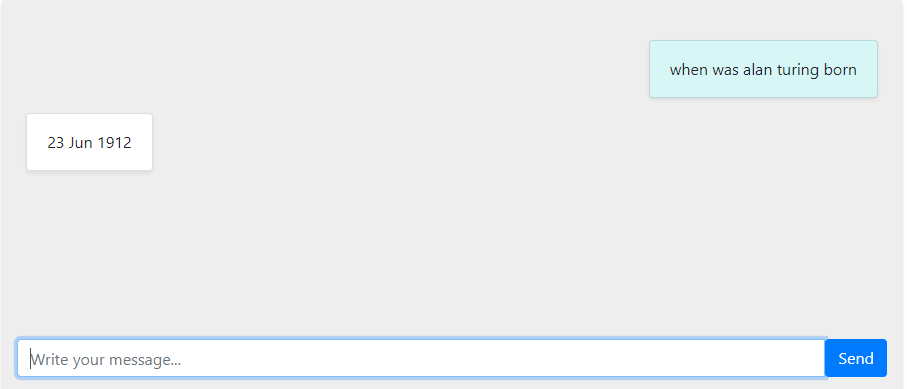
\includegraphics[width=8cm, valign=m]{tests/f7} & Yes \\
		\midrule
		F8 & Person Age Query
		& The user should be able to ask a query about a person's age\newline - 'HOW OLD IS *' and see their age
		& 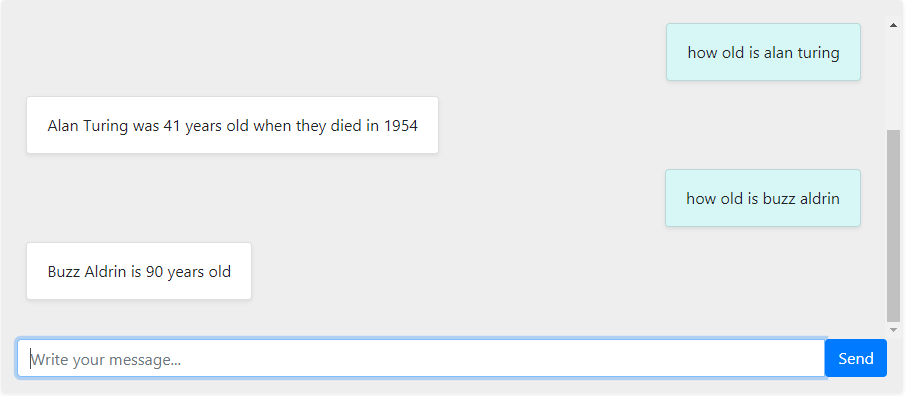
\includegraphics[width=8cm, valign=m]{tests/f8} & Yes \\
		\midrule
		F9 & Person Birthplace Query
		& The user should be able to ask a query about where a person was born\newline - 'WHEN WAS * BORN' and see their birthplace
		& 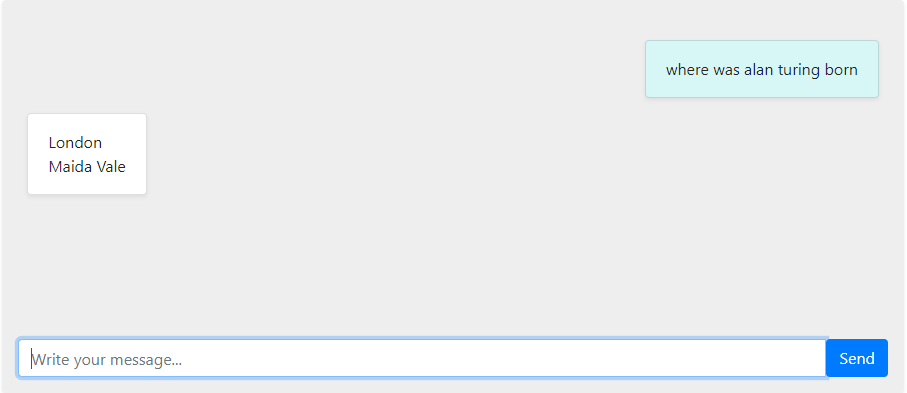
\includegraphics[width=8cm, valign=m]{tests/f9} & Yes \\
		\midrule
		F10 & Person Death Date query
		& The user should be able to ask a query about when a person died\newline - 'WHEN DID * DIE' and see their death date
		& 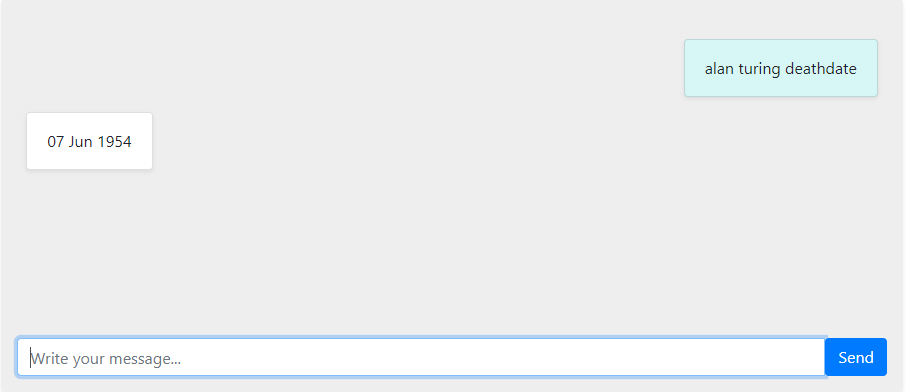
\includegraphics[width=8cm, valign=m]{tests/f10} & Yes \\
		\midrule
		F11 & Person Known For Query
		& The user should be able to ask a query about what a person is known for\newline - 'WHAT IS * KNOWN FOR' and see what they are known for
		& 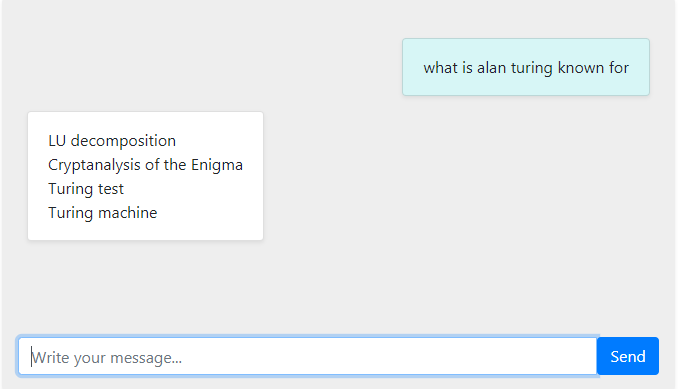
\includegraphics[width=8cm, valign=m]{tests/f11} & Yes \\
		\midrule
		F12 & Person Photo Query
		& The user should be able to ask for a photo of a person\newline - 'WHAT DOES * LOOK LIKE' and see a photo of the person
		& 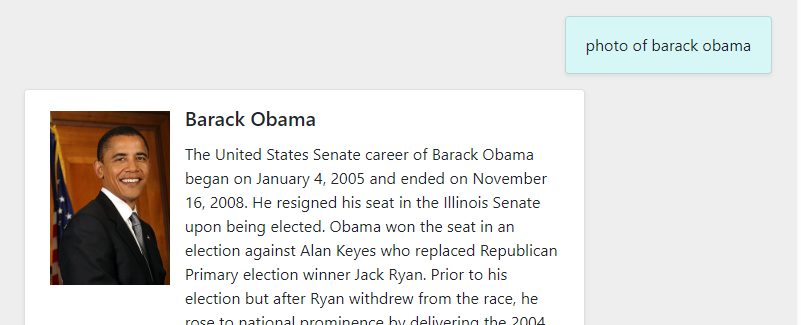
\includegraphics[width=8cm, valign=m]{tests/f12} & Partial\footnote{\label{fn:discuss}Discussed in Section~\ref{subsec:requirementresults}} \\
		\midrule
		F13 & Person Wikipedia Link Query
		& The user should be able to ask for the link to a person's Wikipedia page\newline - '* WIKIPEDIA PAGE' and receive a link to their page
		& 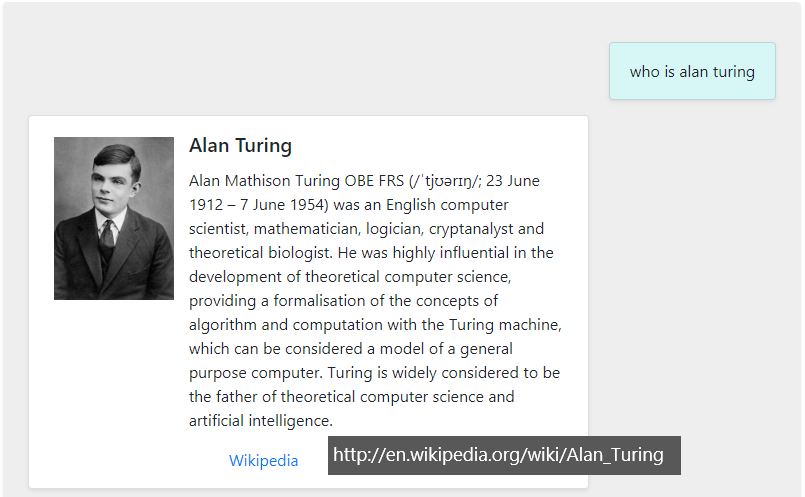
\includegraphics[width=8cm, valign=m]{tests/f13} & Yes \\
		\midrule
		F14 & Country Description Query
		& The user should be able to ask about a country\newline - '[COUNTRY]' and see a description of that country
		& 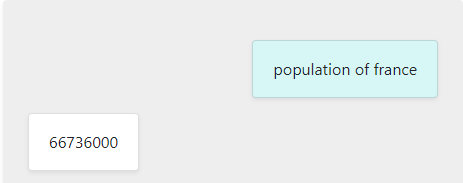
\includegraphics[width=8cm, valign=m]{tests/f14} & Yes \\
		\midrule
		F15 & Country Population Query
		& The user should be able to ask about a country\newline - '[COUNTRY] POPULATION' and see the population of that country
		& 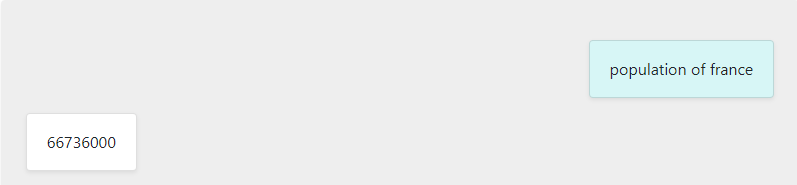
\includegraphics[width=8cm, valign=m]{tests/f15} & Yes \\
		\midrule
		F16 & Country Capital Query
		& The user should be able to ask for the capital of a country\newline - 'CAPITAL OF [COUNTRY]' and see the capital of that country
		& 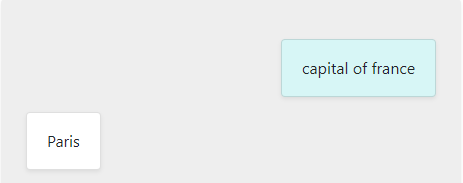
\includegraphics[width=8cm, valign=m]{tests/f16} & Yes \\
		\midrule
		F17 & Person List Query
		& The user should be able to ask for lists of people\newline - 'LIST OF ACTORS' - and see a list of actors 
		& 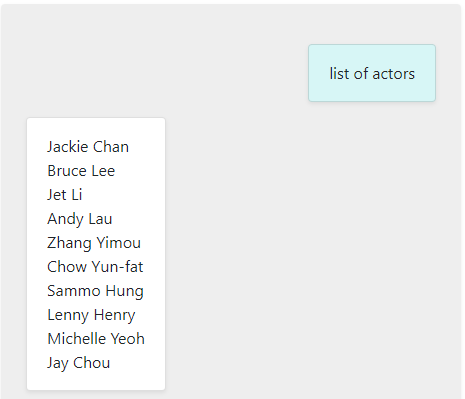
\includegraphics[width=8cm, valign=m]{tests/f17} & Yes \\
		\midrule
		F18 & Person AND Query
		& The user should be able to combine queries\newline - 'LIST OF ACTORS BORN IN 1980 AND BORN IN LONDON'\newline and see a list matching that conditional query
		& 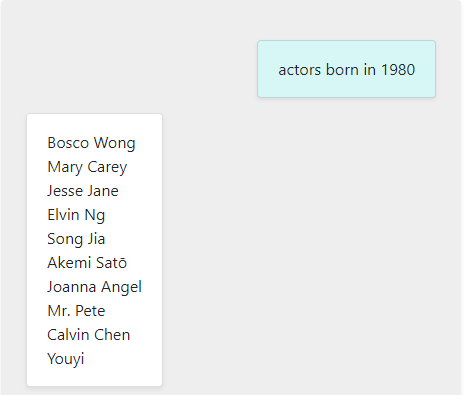
\includegraphics[width=7cm, valign=m]{tests/f18} & No \textsuperscript{\ref{fn:discuss}} \\
		\midrule
		F19 & Context-aware Conversation
		& The user should be able to continue from previous queries using pronouns\newline e.g. 'WHEN WAS HE BORN' and the chatbot should maintain the context of the query
		& 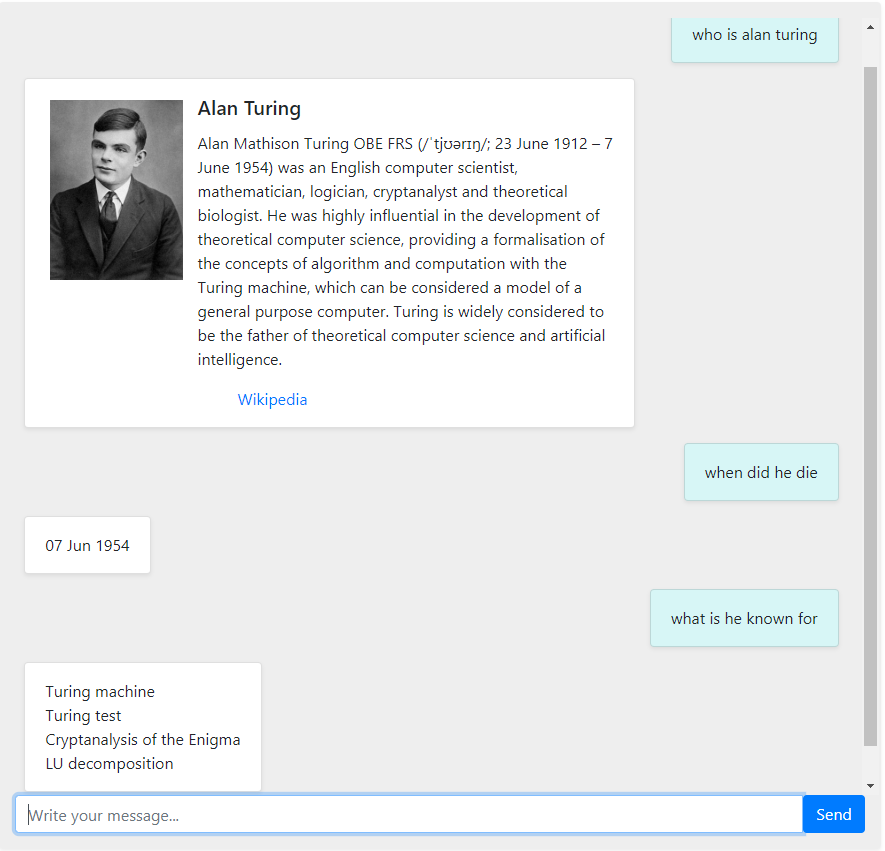
\includegraphics[width=8cm, valign=m]{tests/f19} & Yes \\
		\midrule
		F20 & Chatbot Greeting
		& The chatbot should be able to greet the user
		& 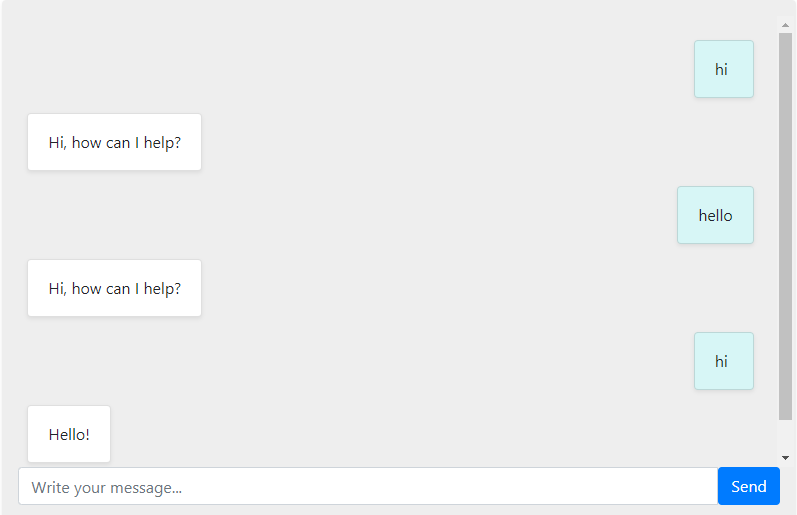
\includegraphics[width=8cm, valign=m]{tests/f20} & Yes \\
		\midrule
		F21 & Chatbot Examples
		& The chatbot should display a list of example queries\newline when asked 'EXAMPLES' or 'WHAT CAN YOU DO'
		& 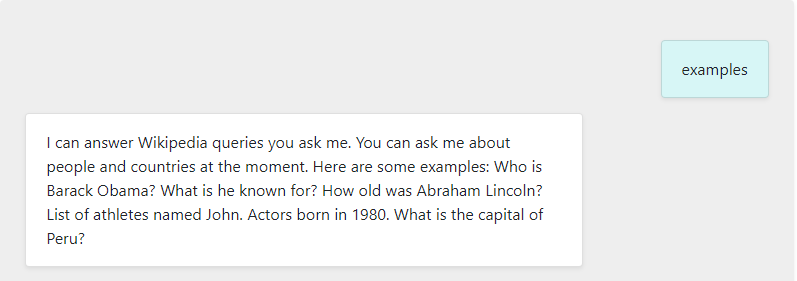
\includegraphics[width=8cm, valign=m]{tests/f21} & Yes \\
		\midrule
		F22 & Chatbot Help
		& The user should be able to receive help from the chatbot\newline on how to use it when asked 'HELP'
		& 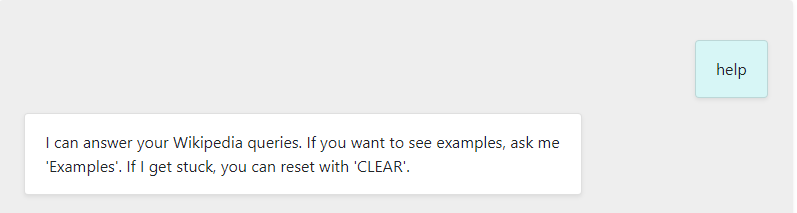
\includegraphics[width=8cm, valign=m]{tests/f22} & Yes \\
		\bottomrule
		\caption{Requirements testing and evidence}
		\label{tab:testreq}
	\end{tabularx}
\end{landscape}

\newpage
\subsection{Performance Testing}
This section focuses on testing the performance requirements of the system, which are:
\begin{itemize}
	\item P1: Web page loads in 5 seconds
	\item P2: Chatbot response in 5 seconds
	\item P3: Application functions without failure
	\item P4: Any errors are logged and the user is informed of an error
\end{itemize}

For P1 and P2, a JavaScript function was used to time the page loading timings. This was repeated ten times using a variety of queries. The results are shown in Figure~\ref{fig:p1}. While there is some variation in loading times for responses -- between 210 milliseconds and almost 2 seconds -- the time never exceeds 5 seconds. The operations that took more time were functions which displayed an image, and also list queries, because they took more time to process and render.

P3 and P4 are naturally harder to test quantitatively, so evidence for that testing falls under the system testing in \ref{sec:systemtesting}. Upon review and in conversation with the test users, it was concluded that P3 was a partial pass, as was P4. The users noticed that occasionally the application would not function as expected, and was not informed about what went wrong. On the server side, errors are not currently logged, mainly due to time constraints. This will become a priority for work in the future.

\begin{figure}[h]
	\begin{center}
		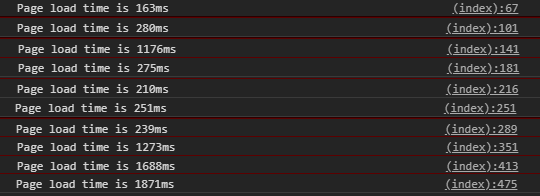
\includegraphics[width=.8\linewidth]{tests/p1}
	\end{center}
	\caption{Performance requirement testing.}
	\label{fig:p1}
\end{figure}

\subsection{Results}
\label{subsec:requirementresults}
The requirements testing for this system have been largely successful. The results from Table~\ref{tab:testreq} reflect this, 20 out of 22 functional requirements being fully implemented. The partial fulfilment of F12 was due to time constraints, where an image is still shown of the person being queried, but this is because these queries have been routed to the summary queries. The failed requirement of F18 was also due to time constraints; the complexity of combining queries using `AND' was not possible to implement in the time frame -- this requirement can be addressed in future work, although in Section~\ref{sec:priority} this was only deemed a low priority requirement. The next phase of testing looks at the system as a whole, with the help of the test users, in order to determine the efficacy of the application.

\section{System Testing}
\label{sec:systemtesting}
Although we have tested the requirements specification, it is important that we assess the accuracy and ability of the system as a whole. For example, we may get a response from the system, but it may not be the result we were expecting. As such, the three testers will be given access to the system in order to answer many unseen questions and assess their output.

In order to formalise this, the users were asked to document the exact query they entered, the result they received, and whether or not it was the result they were expecting, in line with the questions in the specification. They were also asked to ask it further questions beyond the scope of the specification, so that we can establish logical future developments for the system. The format of their testing results is as follows:
\begin{itemize}
	\item Test Number
	\item Requirement (F\#)
	\item Input
	\item Output
	\item Result as expected?
	\item Comments
\end{itemize}
They were asked to test at least 5 queries for each requirement item and document their results with comments. The full test results are given in Appendix~\ref{app:testing}.

The results from this phase are mixed, with some great success and accuracy, as well as some failures and confusion. Looking at the statistics, a total of 156 queries were sent by the users, with 116 expected results, and 40 results not as expected. This gives a total success rate of 74.3\%, which may be considered fairly accurate. However, a lot of these errors derived from either the openness of the questions, or improvements that can be made to the system in the future.

If we focus on the User 1 results (Appendix~\ref{app:testing}), the first issue we encounter is that the chatbot does not disambiguate the query in Test 3. This is a difficult issue because the chatbot has to understand when the user is asking a query when they have not provided any interrogatives in the query. Another issue is when the user does not get the result for the person they were expecting. For example, asking {\it`how old was churchill'} (Test 12), the user expects results relating to Winston Churchill - the same applies for misspelt names (Test 25). To address this, we would need a more advanced system for searching results, and a way for the user to get more results when the initial response is not relevant.

Tests 34, 42 and 46 relate to the sets and maps generated automatically by the system -- `America' does not point to `United States of America' as the user would expect. The same applies for listing `actresses' and `american presidents' -- these have not been linked to the ontology. We can also gain further insight into questions the user wants to ask, as in tests 54-55. When asking about an actor, they may want to see what movies they star in, and their net worth. These queries can be designated for future work on the system.

A similar conclusion can be drawn from User 2. Some issues with phrasing of questions can be implemented in future work, as in Test 25 {\it `what is englands population now'}. The system is fairly successful when talking about countries, aside from formatting of numerical data being hard to read. Further work could be done on listing people by their job -- listing formula one drivers, authors, cricket players, and so on.

The results from User 3 have similar issues that can be investigated, such as an incorrect result for the population of egypt (Test 24).

As we can see from these results, many of the shortcomings of the system follows a similar pattern - country names being shortened, lists of people not being accurate or not including given job titles. However, we can gain some valuable insight into the questions the user {\it wants} to ask, and provides a basis for future work. The next phase discusses the final thoughts from the user, and verifies that the solution works for the user as expected.

\section{User Acceptance Testing}
The final stage of testing is to determine whether the users accept the solution or not. I had individual conversations with the three users, to get some final words of feedback on the system as a whole. While the response was overall positive, and all three users accepted the solution, there were some themes surrounding where the system fell short, and where improvements can be made in the future.

\subsection{UAT Findings}
This list summarises the key findings during this phase, taken from conversations with the three users.
\begin{itemize}
	\item \textbf{Clear and easy to use interface} -- On the whole, the users found the interface to be intuitive to use. One user was fond of the Person summary message which showed the person's photo and Wikipedia link. They noted that it would be useful to have more summary information here like you would find on a Wikipedia page.
	\item \textbf{Formatting of message could be improved} -- All of the users noted in their comments in Appendix~\ref{app:testing} that the formatting of messages could be clearer or be more conversational. This includes the numbers being formatted to include comma separation, or responding to a question in a more conversational way.
	\item \textbf{Not all job types could be used for lists} -- Many users tried to list people by job types that were not generated by the system, including formula one drivers, authors, cricket players, and so on. The users sometimes found it hard to know which titles could be used.
	\item \textbf{Lists were often in a bizarre order} -- Some users noted that the listing provided unexpected results. For example, User 3 Test 36 asked for actors born in 1960 but did not recognise any of the results.
	\item \textbf{Chatbot sometimes got confused} -- When the chatbot did not understand the question or did not have any results, it would often repeat the previous message. Users wanted to see some confirmation that something went wrong, or provide suggestions on how to remediate it.
	\item \textbf{System sometimes returned information about the wrong person} -- This was a common issue that users were having. When they asked for information about a certain person, they were often given results based on a different person with a similar name. They wanted to be able to change this so that they could tell the chatbot to find someone else.
\end{itemize}

\subsection{UAT Future Improvements}
Below is a summary of the suggested future improvements, taking on board the feedback from the test users.
\begin{itemize}
	\item \textbf{Improve the formatting of messages} -- every user agreed that the formatting of the message needed work, especially for country queries, they would have liked to see the number values either rounded or comma-separated. Most users also agreed that putting the answer in context would be a bit clearer, e.g. {\it `The population of India is 1.353 billion'}.
	\item \textbf{Provide suggestions for next questions to ask} -- it would be useful to know what next to ask about the person, and provide clickable buttons to ask that automatically without having to type out the queries.
	\item \textbf{Improve listing functions and add more advanced filters} -- being able to click a person in the list to find out more information would be a useful feature. The users added that the order and contents of the list was often strange, and they would have liked to search by other conditions, such as where they were born. One user noted that they would like to make comparisons between countries too.
	\item \textbf{Expand dataset to more topics} -- Users were happy with the system on the whole but felt restricted as they could only ask limited questions. They wanted to ask anything about countries, bands, cities, sports teams, and so on.
	\item \textbf{Allow for user to retrieve more results if the first result was not relevant} -- The user should be able to provide feedback to the system that the result was not relevant, and be able to select from a list of results.
\end{itemize}

\section{Conclusion}
The testing of the system highlighted some key factors to consider. Firstly, it can be very difficult to anticipate what a user is going to input into the system, especially how queries will be phrased. Secondly, although the users were asked for initial requirements for the system, there were several queries and features that users would find useful in the system, which were only discovered when they started using it. Finally, it is important to remember that this is just an initial system. Improvements can be continually made to the system, especially when adding AIML patterns and synonyms. The next chapter focuses on evaluating the project as a whole. 